% Seminar paper for High-Performance Computing with FPGAs (SS2018)
% Gaurav Kumar Singh <gauravks@mail.uni-paderborn.de>
%
% based on a template by Holger Karl, (c) 2001

\documentclass[12pt,twoside]{article}
\usepackage{url}


%%%%%%%%%%%%%%%%%%%%%%%%%%%%%%%%%%%%%%%%%%%%%%%%%%%%%%%%%%%%%%%%%%%%%%%%%%%%%%
%%%%%%%%% configure these settings and you are good to go %%%%%%%%%%%%%%%%%%%%
%%%%%%%%%%%%%%%%%%%%%%%%%%%%%%%%%%%%%%%%%%%%%%%%%%%%%%%%%%%%%%%%%%%%%%%%%%%%%%
\newcommand{\participant}{Gaurav Kumar Singh}
\newcommand{\affiliation}{Paderborn University}
\urldef{\emailaddress}\url{gauravks@mail.uni-paderborn.de}
\newcommand{\topic}{Accelerating Bioinformatic applications using FPGA based HPC system}


%%%%%%%%%%%%%%%%%%%%%%%%%%%%%%%%%%%%%%%%%%%%%%%%%%%%%%%%%%%%%%%%%%%%%%%%%%%%%%
%%%%%%%%% don't make any other changes in the following   %%%%%%%%%%%%%%%%%%%%
%%%%%%%%% preamble unless you know what you are doing     %%%%%%%%%%%%%%%%%%%%
%%%%%%%%%%%%%%%%%%%%%%%%%%%%%%%%%%%%%%%%%%%%%%%%%%%%%%%%%%%%%%%%%%%%%%%%%%%%%%

\usepackage[english]{babel}
\usepackage[T1]{fontenc}
\usepackage[utf8]{inputenc}
\usepackage{times}
\RequirePackage[style=ieee,doi=true,isbn=false,url=false,mincitenames=1,maxcitenames=3,minbibnames=10,maxbibnames=10]{biblatex}
\usepackage{geometry}
\geometry{a4paper,body={15cm,22cm}}
\RequirePackage{xpatch}
\xpatchbibmacro{textcite}{\addspace}{\addnbspace}{}{}
\xpatchbibmacro{Textcite}{\addspace}{\addnbspace}{}{}
\usepackage{amsmath}
\usepackage{multirow}
\usepackage{graphicx}
\usepackage{paralist}
\usepackage{fancyhdr}
\usepackage{cleveref}
\usepackage[font=footnotesize,labelfont=bf]{caption}
\RequirePackage[margin=0cm]{subfig}
\bibliography{references}
\pagestyle{fancy}
\fancyhead{}
\fancyhead[LE]{ \slshape \participant}
\fancyhead[LO]{}
\fancyhead[RE]{}
\fancyhead[RO]{ \slshape \topic}
\fancyfoot[C]{}

\begin{document}

\title{\topic}
\author{\Large{\participant}\\ \affiliation \\ {\small \emailaddress}}
\date{}
\maketitle
\thispagestyle{empty}

%%%%%%%%%%%%%%%%%%%%%%%%%%%%%%%%%%%%%%%%%%%%%%%%%%%%%%%%%%%%%%%%%%%%%%%%%%%%%%
%%%%%%%%% here starts the actual text                     %%%%%%%%%%%%%%%%%%%%
%%%%%%%%%%%%%%%%%%%%%%%%%%%%%%%%%%%%%%%%%%%%%%%%%%%%%%%%%%%%%%%%%%%%%%%%%%%%%%

% Abstract gives a brief summary of the main points of a paper:
\begin{abstract}

 The Human Genome project was completed in the year 2003 and vast avenues 
 of research were opened for developing and enhancing Genomic analysis techniques. The Genomic
 research greatly relied on bioinformatics capabilities with the vast sequence
 database now available. Improvements to the computational speed were necessary and required identification of
 techniques to increase the processing capabilities of the existing algorithms and tools and develop
 new techniques to utilize advancements in computing.
 
 Utilization of FPGA to reduce processing times by huge factor compared to other CPU and GPU based techniques
 is proving an important step towards this goal. Similarly, the use of high performance clusters has shown
 to be very effective for large sequence analysis. Combining these technologies together possess great benefits
 for speeding up the analysis of the huge databases further. This paper will capture the requirements of bioinformatic
 application and present FPGA based acceleration technique for the \textcite{smith_identification_1981} algorithm.
 Initially we look at bioinformatics application areas where FPGA and HPC system are beneficial. Then the paper describes
 some of the algorithms which can be accelerated using FPGA and HPC in a heterogenous system. The last part presents
 a system and evaluation results in terms of speedup compared to existing systems and tools.

\end{abstract}

% the actual content, usually separated over a number of sections
% each section is assigned a label, in order to be able to put a
% crossreference to it

\section{Introduction}
\label{sec:introduction}

Humans quest to understand the basic biological processes lead to development of research areas such as
biochemistry and biotechnology. Research of biological molecules from multiple decades have helped us to understand
the existence of DNA and genome which defines the existence and behaviour of a living organism.
On the other hand the advancement in computer technologies and increased use in healthcare, biomedical
and computational biological research has helped find cures and medical treatments for many complex health
issues and save many lives over the years.

In efforts to increase the knowledge of genomes, the field of Bioinformatic was created. Bioinformatic majorly involves
the study of biological molecules (biomolecules) which build up the cells of the living organisms. As with the other biological fields,
bioinformatic aims at utilizing the capabilities of the computer science to build and analyse molecular sequences (genes) of DNA.
In this direction, The \emph{Human Genome Project}\footnote{\url{http://https://www.genome.gov/}}  was started in late 1990 and was
completed in 2003 successfully. "A 2.91-billion base pair (bp) consensus sequence of the euchromatic portion of
the human genome was generated by the whole-genome shotgun sequencing method"\cite{venter_sequence_2001}. This was a huge
step but also presented the problem of huge processing times for analysis of such a large database of genome for extracting any
useful information. The existing algorithms for database searches such as dynamic programming Smith-Waterman \cite{smith_identification_1981}
for local similarity estimation and heuristics-based BLAST \cite{altschul_basic_1990} were limited by
high computation times. The main factor for this was the limited processing capabilities of the computing units
on which the algorithms were running.

Various methods in the past decades have evolved to provide higher computing and data processing capabilities for various application domain.
The earliest method being hardware acceleration provided by symmetric multiprocessing which allows distribution of computing to different processor
sharing a common memory. The next major acceleration achieved has been the development of high performance computing clusters (HPC).  HPC
system work by splitting and distributing the problem over multiple similar processing units, known as nodes. Each of the node
consists a high-speed processor with multiple cores with shared memory. The nodes in the clusters are connected to
each other with high-speed Ethernet connections for exchange of data and control information. Each node can be used to
process a sub-set of the data parallelly decreasing the overall computing time for the problem. Due to such benefits, these techniques were
introduced for Bioinformatic algorithms to speed up processing time.
Implementation of the famous Smith-Waterman algorithm on HPC systems is presented in \cite{boukerche_parallel_2005,martins_multithreaded_2000}.
Multiple parallel implementation for BLAST such as mpiBLAST \cite{darling_design_2003} are available as well, which prove
to be more time efficient. \textcite{schmidt_massively_2002} showed how such improvements can be used to create a parallel system which
helps to speed up the molecular sequence analyse.

Another step in increasing the processing capabilities of the clusters was utilization of GPU. GPUs allow offloading
the vector based arithmetic operations for large datasets. They prove to be excellent accelerators for reducing
the processing time with large amount of data. \textcite{liu_cuda-blastp:_2011} have presented such a system which can perform
10 times faster compared to serial versions of BLAST \cite{altschul_basic_1990}.

Though the parallel implementation with CPU and GPU help in achieving faster processing time, its heavily dependent
on the size of the cluster. Also, the speedup highly depends on the size of the problem. These reasons
made researchers to look for techniques which can reduce the execution times of the algorithm by use of hardware-based
accelerators. Such accelerators aim at fast processing of each operation leading to shorter execution time. This is where the FPGA has 
helped a lot by providing opportunities to implement the algorithms directly in the hardware. The flexibility
of FPGA makes them very useful to design application specific acceleration hardware and
re-use them for different kinds of problems. Currently a lot of accelerators are available from which, the bioinformatic
community is benefiting. This paper would discuss some of these implementations and give an overview of how
such accelerators are integrated with the HPC clusters to build heterogenous systems which are used to
achieve very high processing speeds to reduce the time from days to hours for some bioinformatic application.

The rest of the paper is divided into 3 sections. Section 2 introduces the bioinformatic application domain giving
details of algorithms and tools popularly used. Section 3 will present the optimization techniques for genome
comparison by FPGA and heterogenous systems and the last section presents results achieved by such optimization
for some of the current systems.

\section {Bioinformatic and its applications}
\label{sec:bioapplications}
Bioinformatic can be considered as an amalgamation of molecular biology and computer science.
As described by \textcite[chapter 8]{gokhale_reconfigurable_2010}, it mainly focuses on analysis
and management of biomolecular data to support research works for identifying causes of diseases and
specialized drug discovery. Apart from genome assembly and analysis, bioinformatic also concentrates
on protein classification and structure prediction, gene prediction and phylogenetic prediction.

Genomic data is mainly built up from DNA or protein sequences. DNAs are built from a sequence of
nucleotide base pairs(bp). The four nucleotide molecules adenine (A), thymine (T), cytosine (C), and guanine (G)
form these base pairs and are always arranged such that adenine (A) pairs with thymine (T) and
cytosine (C) pairs with guanine (G). These bp can arrange in different ways and different lengths to build up the DNA
sequences. The DNA sequences form the gene, the entity known to be responsible for some specific functionality,
or the complete genome of the organism. The sequence of DNAs are stored on computers as string containing only the
alphabets A, T, C and G representing the respective nucleotide molecules. Similarly the protein molecules
are also represented by 20 \{A, C, D, E, F, G, H, I, K, L, M, N, P, Q, R, S, T, V, W, Y\} alphabets assigned
based on the amino acids composition.

\textcite[chapter 2]{mount_bioinformatics:_2004} describes the complex DNA sequencing process which involves
extraction of the DNA fragments by using polymerase chain reaction (PCR) and tagging them for identification.
Genome sequencing involves a laborious process of generating smaller sub-clones of the original sequence and
then identifying overlaps to assemble the sequences. Small sequences are easy and cost effective to identify
and record but identification of the complete genome with similar techniques can be very costly. To reduce
the cost the small sequences are fed into the computer to create sequence databases using the string
representation of the bp and then computer programs are used to assemble them by identifying overlaps.
Genome databases collect such new sequences and provide them to researchers for analysis. The focus
of the analysis is identification of similarity between genomes of different organisms and mapping
functions to the gene. Such similarities help to identify and build the divergence tree of species
through years of evolution. The gene mapping is also important to understand how the body behaves and can
be used to study effects of different chemicals during drug trials.

All these studies require some form of string matching to compare or identify subsection from the huge
databases. As string comparison involved in the algorithms can be done with simple mathematical
operations over long operands, they can be easily mapped on simple circuits on the FPGA. As these
operations does not involve any complex floating point operations FPGA are suitable to speed up the
processing with dedicated hardware.

The rest of this section will explain the Bioinformatic application areas where FPGAs based accelerators
can be used to speed up the processing. Some of the algorithm will also be presented to understand their
functionality and usage in the bioinformatic domain.

\subsection{Application areas}

As highlighted earlier, the FPGAs can be a suitable target to accelerate the simple processing requirements
of the bioinformatic domain and speed up the processing by huge factor. In this subsection, some of the
application areas where FPGAs are suitable will be explained.

\subsubsection{Genome Assembly/sequencing}

Identification of the complete DNA sequence or the Genome of an organism has been one of the most common
application of bioinformatic from the early 1990. The identification of complete DNA sequence involves
forming small fragments of subclones of the large sequences and then re-arrange the fragments by comparing
the ends to find overlaps between the fragments\cite[Chapter 2, Genome sequencing]{mount_bioinformatics:_2004}.
This method is known as the shotgun sequencing and has been used to create the complete genomes of many organism
including human genome as shown in \cref{fig:sequence}.

\begin{figure}%
    \centering
    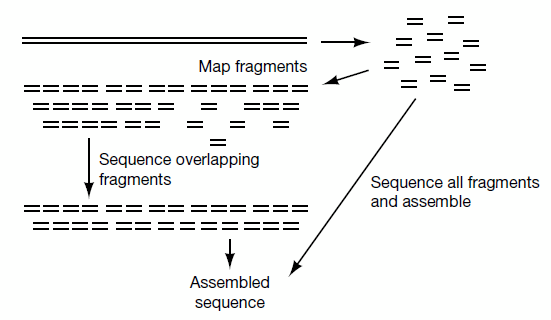
\includegraphics[width=0.8\textwidth]{fig/sequence}
    \caption{Sequencing process \cite[Figure 2.4]{mount_bioinformatics:_2004}}
    \label{fig:sequence}
\end{figure}

The main idea involved is comparison of overlap regions in the fragments to arrange them in the sequence. This
is mostly achieved in computers by using pairwise comparisons of the strings for the fragments and identifying
the similarities towards the end. Such comparison which mostly involve simple comparison operation of some
fixed number values can be easily implemented in FPGA with high accuracy.

\subsubsection{Genome comparison}

Another important bioinformatic application is comparison of genomes of different organism to identify similarities
in gene content, gene location and gene number. As the number of fully identified genomes is increasing at rapid pace,
the researchers focus a lot to identify these similarities which help to understand the evolution trend of the organisms.
If the number of identified gene and their functionality in different genomes are similar to a large extent, this can be
easily used to conclude that organism have common evolution history. Similar genes are often mapped to different functionality
which is important indication of divergence during the evolution of the organisms. 

The genomic comparison also involves comparison of strings to identify similar pieces but on a longer length of the whole
genome which can be in 100 thousand bp. As the sequences can be long, FPGAs can be used for acceleration by decreasing the
computation time, compared to single processor solutions, and produce results much faster.

\subsubsection{Gene prediction}

One of the important aspects of DNA sequencing is to identify the sequences which perform a specific functionality
within the organism. Such sequences are called genes and an organism's genome can be divided into 100 of gene
segment, each of which can be mapped to some specific functionality. The functionality of the gene is identified
by predicting the sequences which encode some proteins molecule. Such sequences are identified by looking for
open reading frames (ORF) which are sequences of bp which contains a codon encoding one of the amino acids.

Gene prediction algorithm use the known databases of amino acid sequences to identify similar patterns
in the genome and tag them with the identified amino acid. The amino acid sequences are used to identify
the resulting protein structure and predict it by searching for similar ones on known organism genome. The searches
for gene prediction involve multiple databases and can be time consuming if whole database is required to be
searched element by element for accuracy. FPGAs . The exhaustive searches can be parallelized over multiple systems
to reduce the overall time. Models based analysis which is popular, can benefit from custom FPGA as it modification to
models can be updated easily still achieving lower processing times.

\subsubsection{Protein domain databases}

As the protein identification is the most common approach for predicting similarities in the sequence, capabilities
to perform quick search on the databases are important. The proteins differ based on the functionality they perform in
the cell called as domain. It is important to categorize the proteins in to specific domain based on their functionalities
and create some models which helps to fetch the target proteins from databases faster. There are various methods and models
which accomplish this such as HMMER based on HMM models.

The algorithms basically involve multiple sequence alignment and require iterations to train the models to enhance
the protein identification. Such systems can be targeted on FPGA which provide the capability for dynamic remapping
which can be used during training.

\subsubsection{Phylogenetic tree}

The phylogeny of the organism is used to identify the relationship between two organisms by analyzing the differences in the
functionality of the gene location and gene functionality of similar genes. The gene location-based analysis tries
to identify the distance between the similar gene on different organism to estimate the generation difference among the
species. Similarly, the functionality-based analysis identifies the difference or similarity in the functionality of
similar or different gene sequence by analyzing the similarities in the families of proteins they encode.
Tree based representation are used to present these deviations, which forms the evolutionary path of an organism. Gene with
smaller distance would have close common ancestor branches compared to larger distances which will be seen by generations gaps.
The differences in the protein families are similarly represented. Two sequences which produce proteins performing similar
functionality would lie on neighbouring branches.

The analysis in the Phylogenetic uses string comparison to identify the similarities from the DNA or protein sequences and
requires a lot of string comparison algorithm. The FPGA can be used to accelerate the string comparison and database searches
to compute the differences in distance and functionalities.

\subsection{Algorithms for sequence comparison}

Analysis in the bioinformatic mostly involves comparison of string sequences of DNA or protein
to identify similarities based on the applications. The comparison results help then to categorize,
and associate identified sequences with specific functionalities (Gene Prediction) or compare with
known DNA Gnome (Gnome comparison) to for evolutionary similarities (Phylogenetic tree).

Though the DNA and protein sequences are represented as string, the standard string comparison algorithm
can't be effectively used because DNA sequences are not static due to the mutation caused over time.
Sequence alignment is therefore used which performs the comparisons by considering the three
mutational operations insertion, deletion and substitution during the comparison. Main idea of sequence
alignment is to assign scores for individual alphabet comparison considering the mutation and use the
sequence which has highest score. There are three categories of algorithms which use sequence alignment
and are used widely for different application domains in bioinformatic.

\begin{itemize}
    \item \textbf{Dynamic Programming (DP)} based algorithms are iterative and compute the alignment cost for individual alphabets
    to fill the similarity score in a matrix. The first algorithms were proposed  by \textcite{needleman_general_1970}
    in their paper in 1970 followed by \textcite{smith_identification_1981} in year 1981.    
    \item \textbf{Seed-based Heuristics}:  DP algorithm are mathematically accurate but are time consuming which led researchers
    identify faster algorithms based on heuristics which were faster but maintaining similar accuracy. The main idea of
    heuristics based algorithm is the assumption that important similarities which are small (seeds) are conserved in
    the same way. The algorithms FAST \cite{pearson_improved_1988} and BLAST \cite{altschul_basic_1990}
    were initial algorithm proposed which used seeds to decrease the computation time for sequences
    and are popular for various applications.
    \item \textbf{Languages Models and Profiles}: Once a vast range of genomic strings are identified by experiments or
    by genome sequencing algorithms, building a model to represent the common features among the strings is useful.
    Models help to decrease the search time of a string in databases by categorizing them based on domains. 
    HMM proposed by \textcite{hughey_hidden_1996} "is a statistical model which considers all the possible combination
    of matches, mis-matches and gaps to generate an alignment of a set of sequences" \cite{mount_bioinformatics:_2004}
    and is used to optimize protein database searches with some additional modifications.
    
\end{itemize}

The rest of section will describe the techniques involved in DP algorithms.

\subsubsection{Dynamic Programming}
\label{subsec:dp}

As \textcite[Chapter 3]{mount_bioinformatics:_2004} describes alignment is a procedure of comparing bp of two of more DNA sequences
to identify the individual and sequence of bp which match in each of the strings. The alignment can also be extended to
identify and estimate the cost of transformation of individual strings. Alignment is performed at two
levels. The global alignment is stretched over the entire sequence whereas the local alignment limits to strong matches within
the sequence as shown in \cref{fig:localglobal}. Local alignment is useful when the string to be compared are long.
\textcite{gokhale_reconfigurable_2010} states the three condition which can occur while estimating the alignment of sequences
at a given position. An example to show the mutation and corresponding global alignment of the original and the mutated
string is shown in \cref{fig:alignment}:

\begin{figure}%
    \centering
    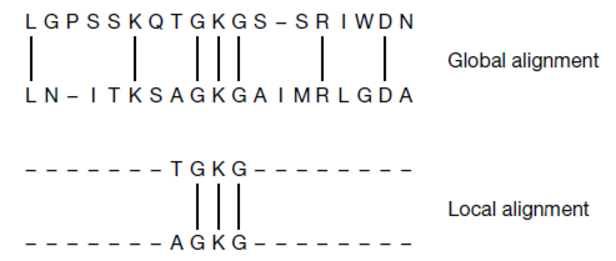
\includegraphics[width=0.6\textwidth]{fig/localglobal}
    \caption{Distinction between local and global alignment \cite[Figure 3.1]{mount_bioinformatics:_2004}}
    \label{fig:localglobal}
\end{figure}

\begin{itemize}
	\item a match occurs when the same character 'x' is present in both strings
	\item a mismatch, also called a substitution, when there are two different characters 'x' and 'y'
	\item a gap, when there is an insertion of one character in only one string, or symmetrically a deletion in the other string
\end{itemize}

\begin{figure}%
    \centering
    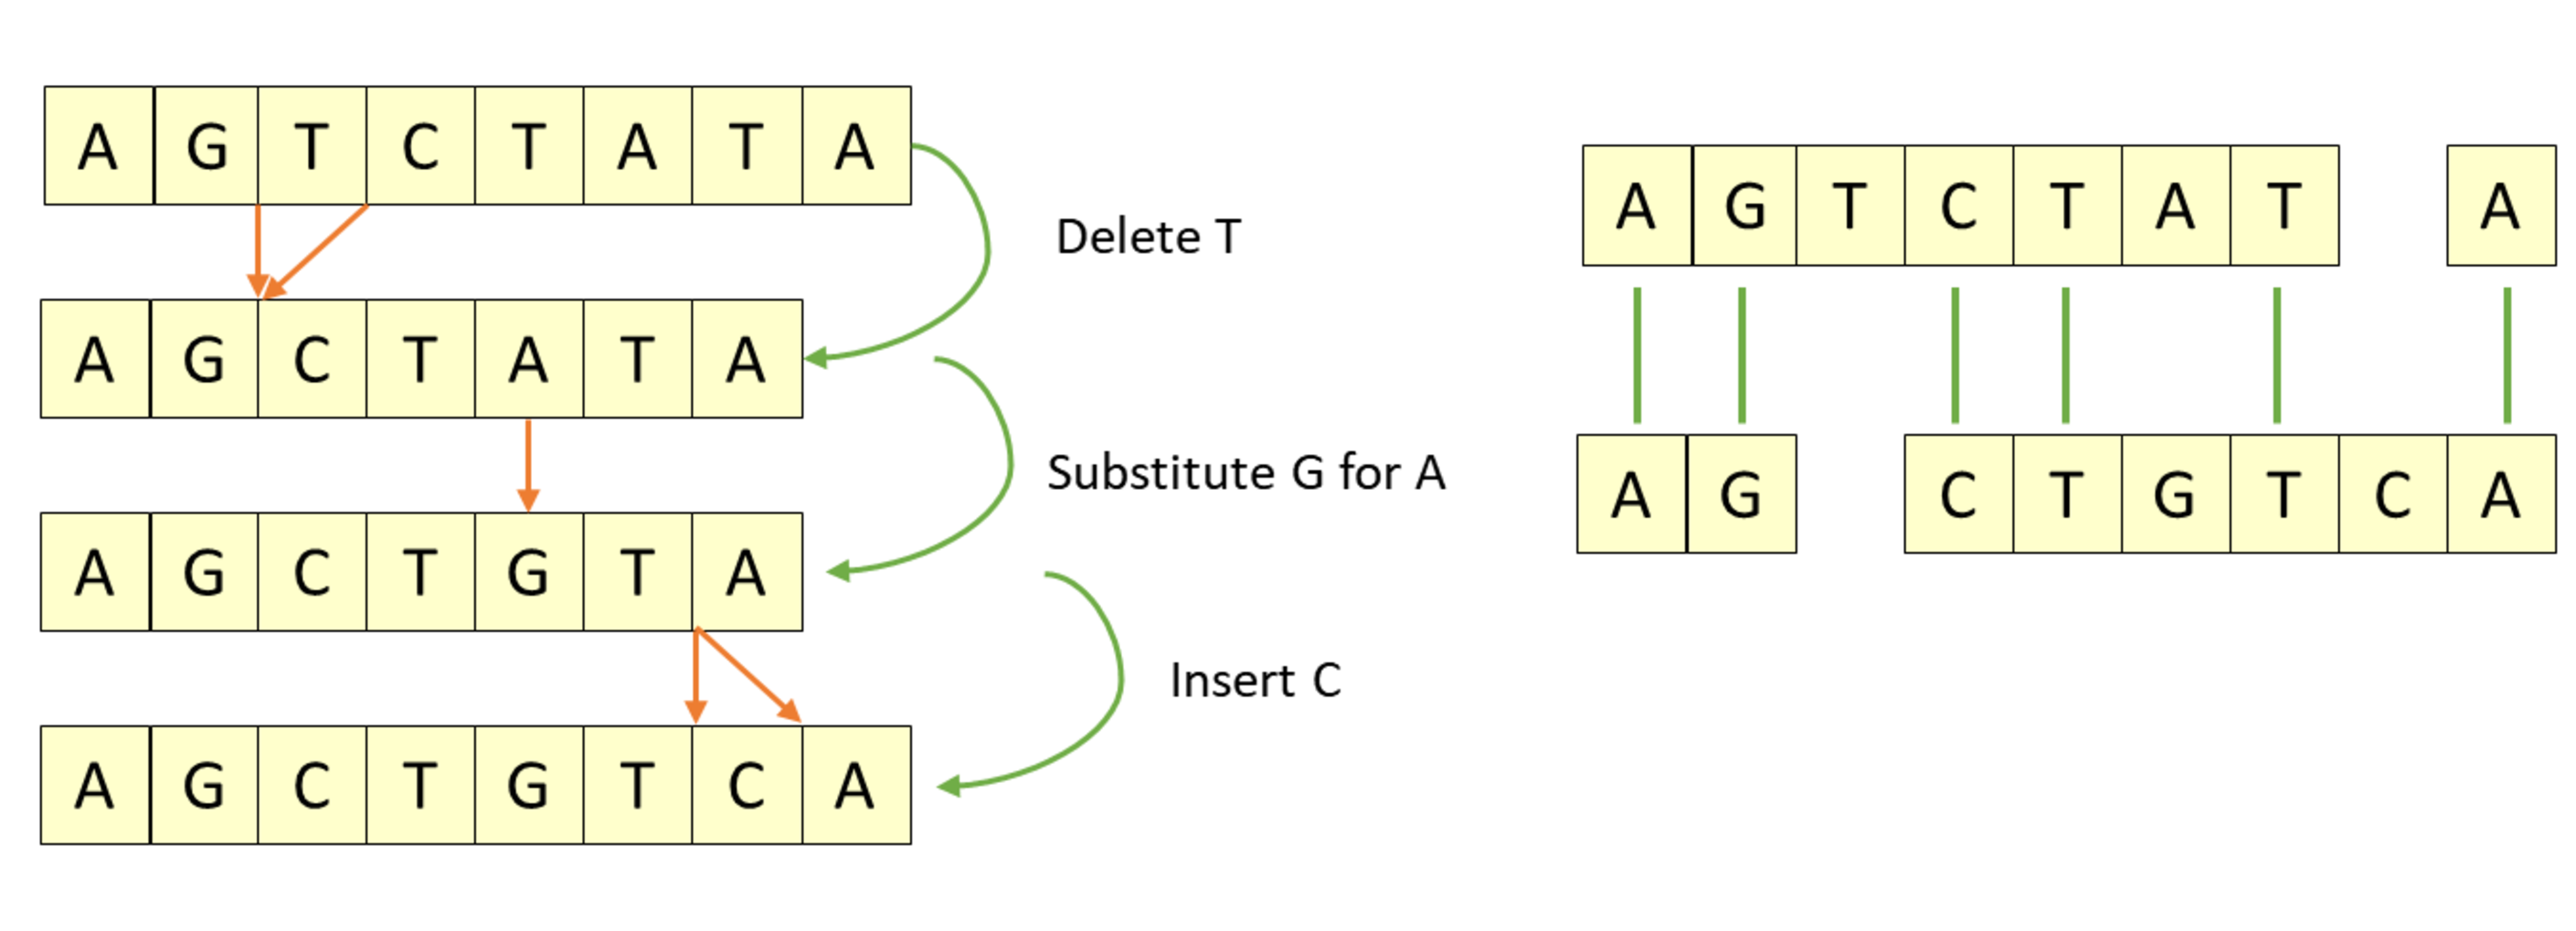
\includegraphics[width=0.8\textwidth]{fig/alignment1}
    \caption{Mutation steps and corresponding alignment of strings identifying the 6 matches,
    2 gaps (T/-,-/C) and 1 mismatch (A/G)}
    \label{fig:alignment}
\end{figure}

Formally considering two string $ X = \{x_1, x_2, ..., x_n\} $ and $Y = \{y_1, y_2, .... y_n\}$
and H(i,j) maximum similarity score at position i, j and $ g_{penalty} $ is the penalty for a gap in the sequence
then the global alignment of the strings can be given by calculating H(i,j) using the Needleman-Wunsch equation \cite{needleman_general_1970} as 

\( \forall i :  H(i,0) = g_{penalty} \times i \) \,\,\,\,\,\,\, \( \forall j :  H(0,j) = g_{penalty} \times j \)

\( \forall i,j,ij \neq 0: \)

\[ H(i,j) =  max
\begin{cases}	
	H(i - 1, j - 1) + d(x_i, y_j) & \quad \text{(match or substitution)} \\
	H(i - 1, j) - g_{penalty} 	  & \quad \text{(insertion)}\\
	H(i, j - 1) - g_{penalty}     & \quad \text{(deletion)}
\end{cases}
\]

The local similarity which is defined for the most similar pair of sub-sequences ending at $x_i$ and $y_i$ is given by
Smith-Waterman \cite{smith_identification_1981} equation as follows:

\( \forall i,j :  H(i,0) = H(0,j) = 0 \)

\( \forall i,j,ij \neq 0: \)

\[ H(i,j) =  max
\begin{cases}
	0							  & \quad \text{(local align. starts here)} \\
	H(i - 1, j - 1) + d(x_i, y_j) & \quad \text{(match or substitution)} \\
	E(i,j)	  & \quad \text{(insertion)}\\
	F(i,J)    & \quad \text{(deletion)}
\end{cases}
\]
where
\[
E(i,j) = max \begin{cases} H(i - k, j) - g_{penalty}(k), & \quad for \,\, 0 < k < i, \end{cases} 
\]
\[
F(i,j) = max \begin{cases} H(i,j - l) - g_{penalty}(l), & \quad for \,\, 0 < l < j, \end{cases}
\]

The scores produced for the alignment of each alphabet is placed in a matrix and back traced from the highest
score to identify the alignment. An example of local alignment calculation is shown in \cref{fig:alignexample}
\begin{figure}%
    \centering
    \subfloat[Alignment]{\label{fig:swexample_a}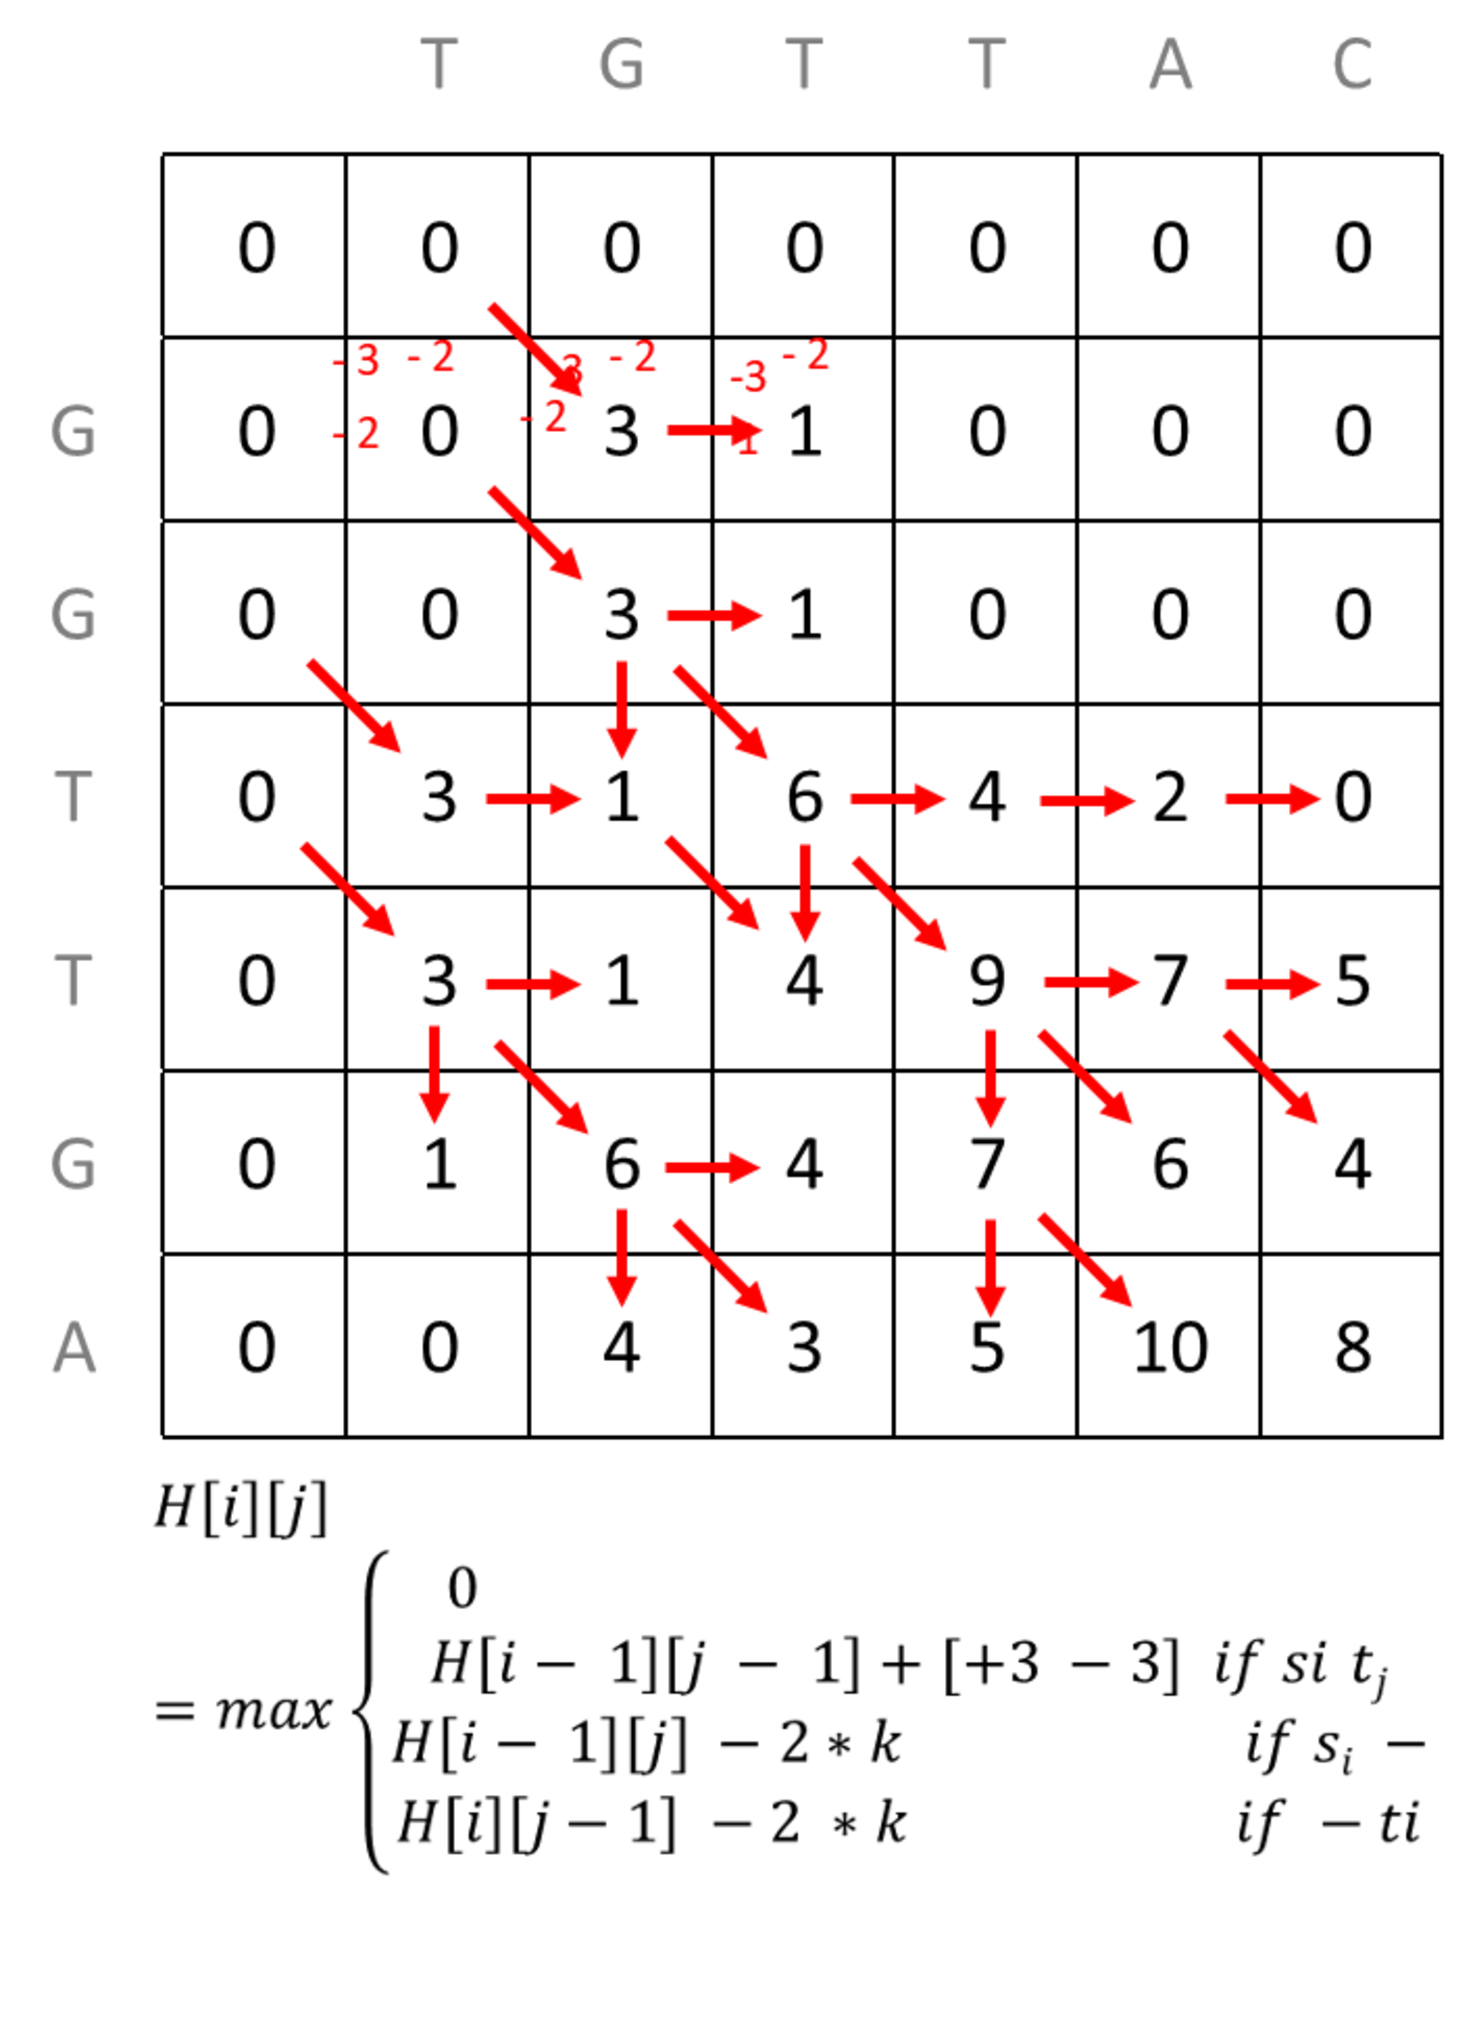
\includegraphics[width=0.46\textwidth]{fig/swexample_a}}\qquad
    \subfloat[Back tracing]{\label{fig:swexample_b}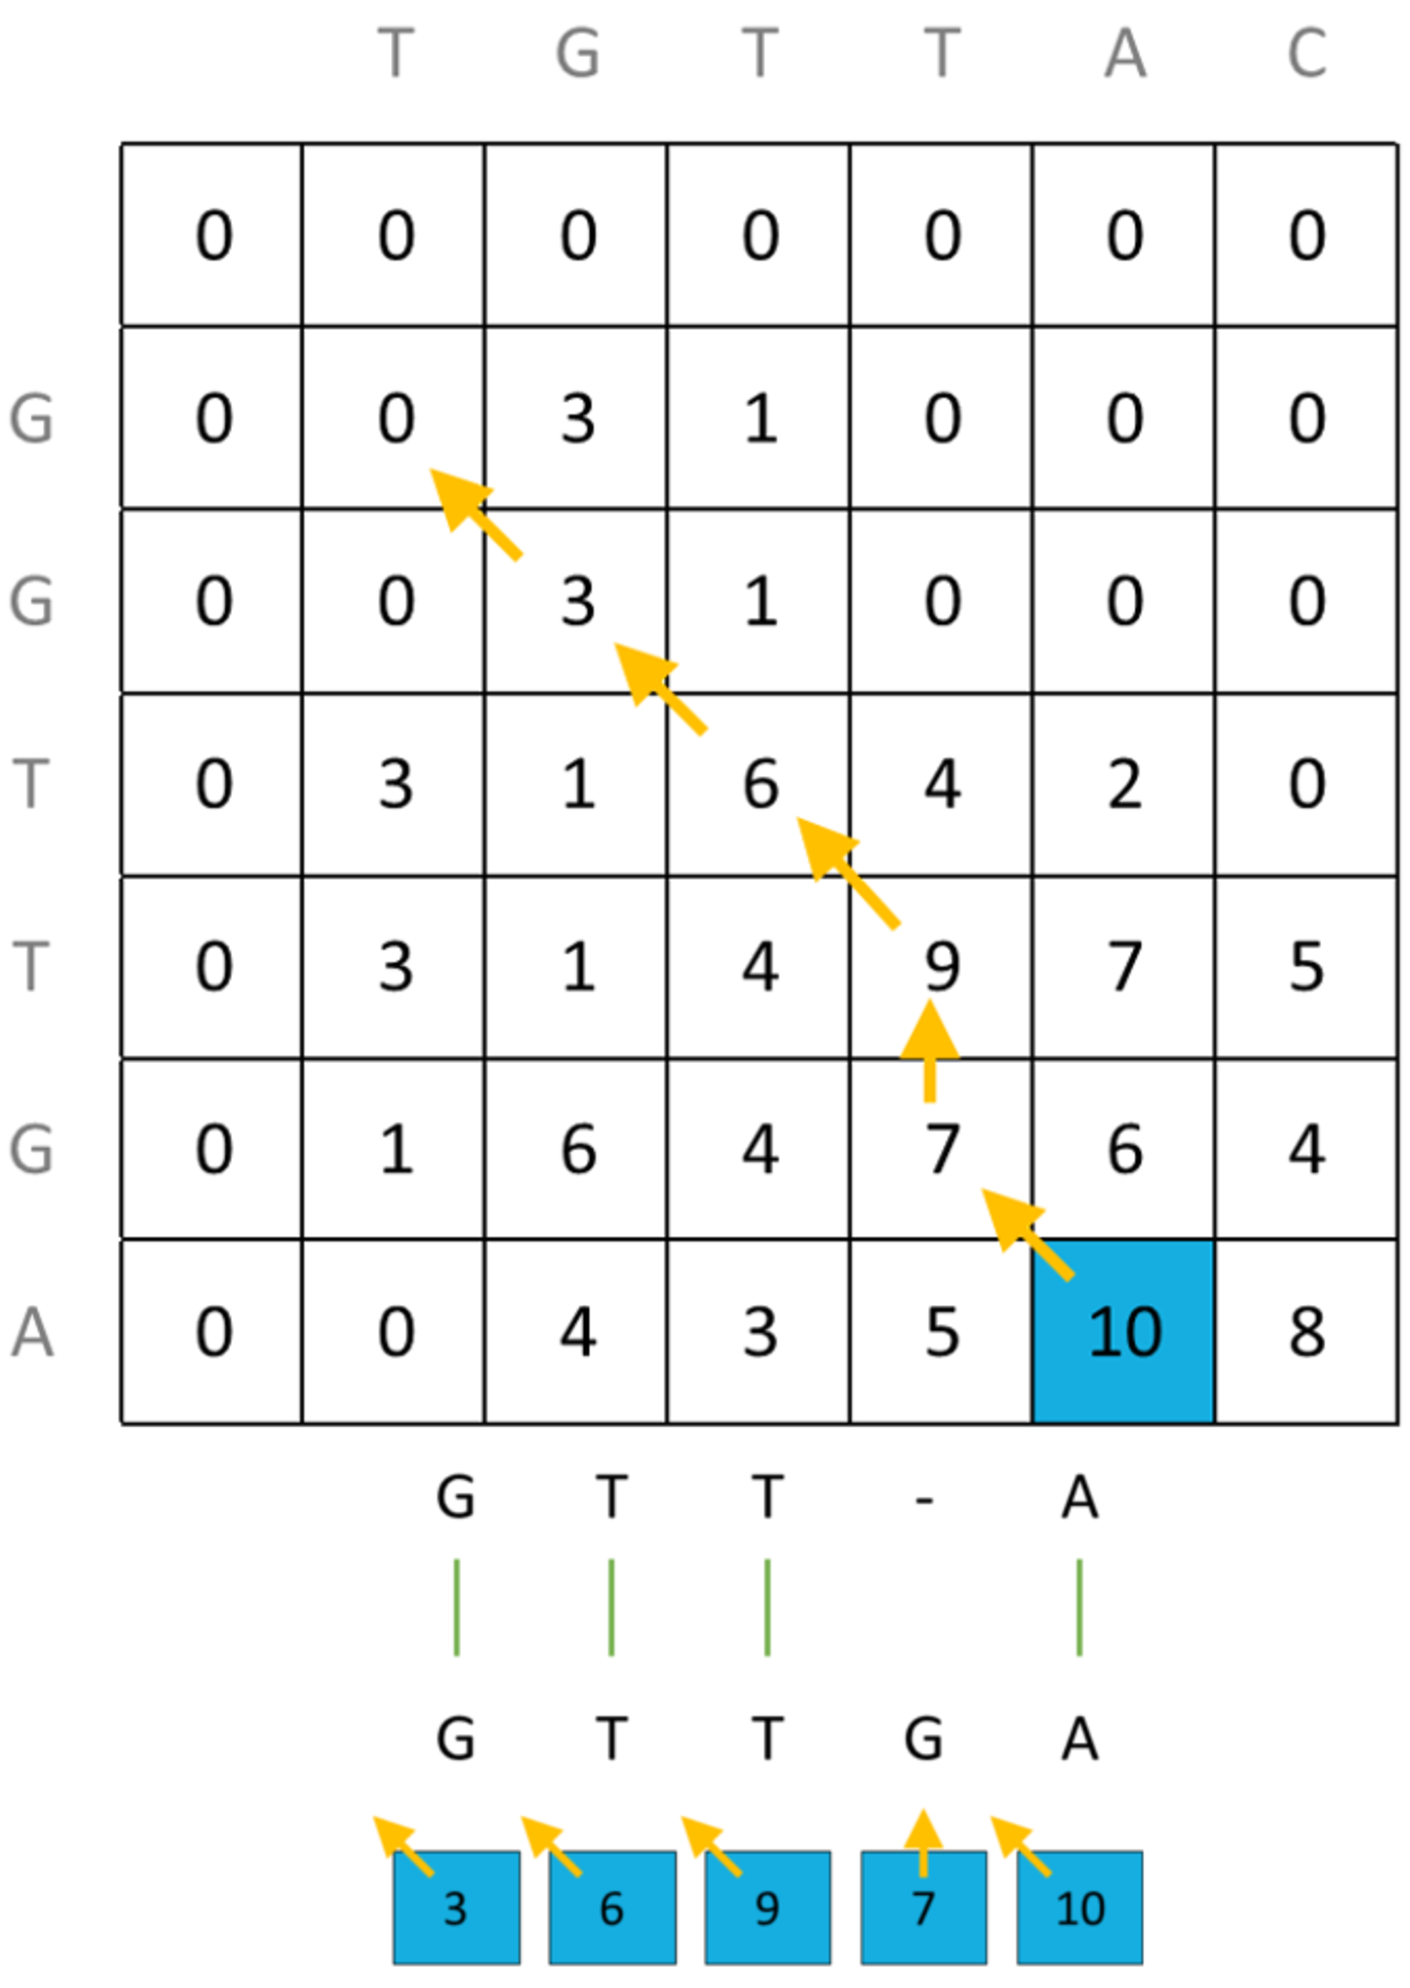
\includegraphics[width=0.45\textwidth]{fig/swexample_b}}
    \caption{Example of local alignment computation with the SW equation (a) Scores are +3 for a match,
	-3 for a mismatch, and -2 for a gap. The red arrows are the dependencies that
	lead to the maximum of each (i, j) cell and reveal the best alignment (b) Back tracing to get the alignment string}
    \label{fig:alignexample}
\end{figure}

\section{Optimization of Genome database search algorithms}
\label{sec:designtech}

The \cref{sec:bioapplications} introduces the application areas and highlights the possibilities for using FPGA to optimize some of the application
areas. This section will present a FPGA based accelerator design for the popular dynamic programming Smith-Waterman algorithm and 
describe a heterogenous system which uses the accelerator to achieve faster database search.

\subsection{FPGA accelerators for Smith-Waterman}
\label{subsec:fpgaaccelerator}

The string alignment achieved by Smith-Waterman (SW) is highly dependent on the size of the search string and size of the databases.
As the size of the databases has been increasing rapidly with identification of new sequences, the processing time for the algorithm
increases similarly. As SW is very accurate and important for the bioinformatic community, various accelerators have been developed
to use it efficiently. Most of the acceleration is achieved by using parallel computation of the similarity score. The
parallelization can be achieved by either splitting and distributing the search database over multiple processors \cite{martins_multithreaded_2000, boukerche_parallel_2005, schmidt_massively_2002, rucci_smith-waterman_2014}
or by passing the database string via a systolic comparison array. The FPGA based system mostly accelerate the processing by 
building hardware systolic cells which allow parallelizing the computation on the anti-diagonal of the score matrix
as shown in \cref{fig:antidiagonal}. In this section we look at the FPGA based systolic accelerator designed by \textcite{oliver_hyper_2005}.

\begin{figure}[h]%
    \centering
    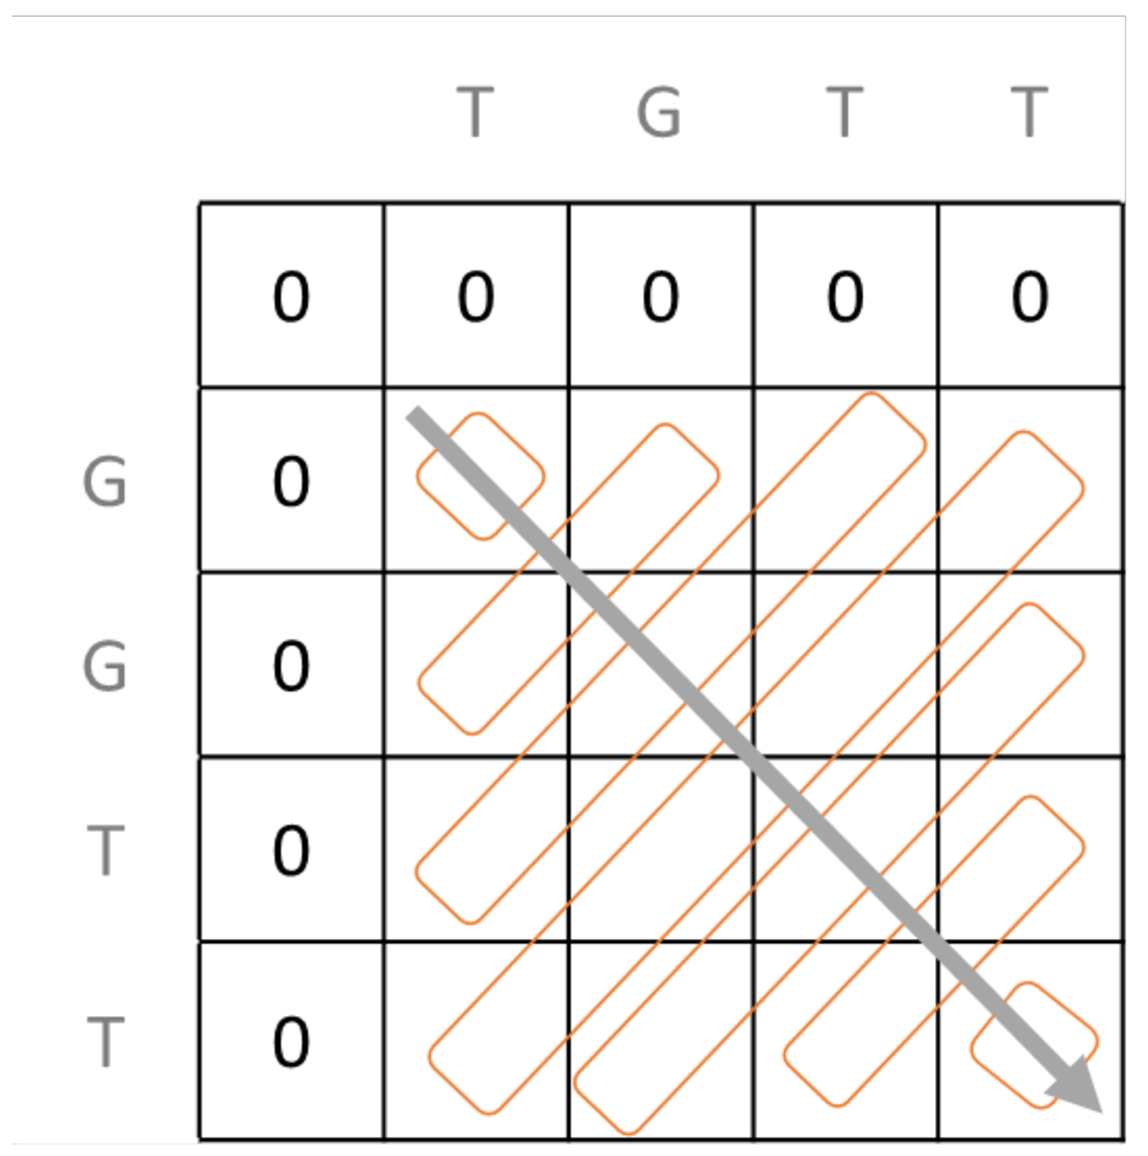
\includegraphics[width=0.4\textwidth]{fig/computation}
    \caption{Parallel computation of similarity score along the anti-diagonal of score matrix}
    \label{fig:antidiagonal}
\end{figure}

\subsubsection{Systolic cells on the FPGA platform}

Calculation presented in \cref{subsec:dp} can easily be mapped to an array of processing elements (PE) of an FPGA creating systolic cells.
Each PE can be initialized by the single character of the search string and then shift the sequence of string from the database systolically
through the array as shown in \cref{fig:systollicarray}. Considering the query string size of M and K be the size of the sequence string to be
searched, the PEs can to complete the comparison in $ M + K-1 $ steps with M PEs instead of $ M \times K $ required for a sequential processor.

\begin{figure}[h]%
    \centering
    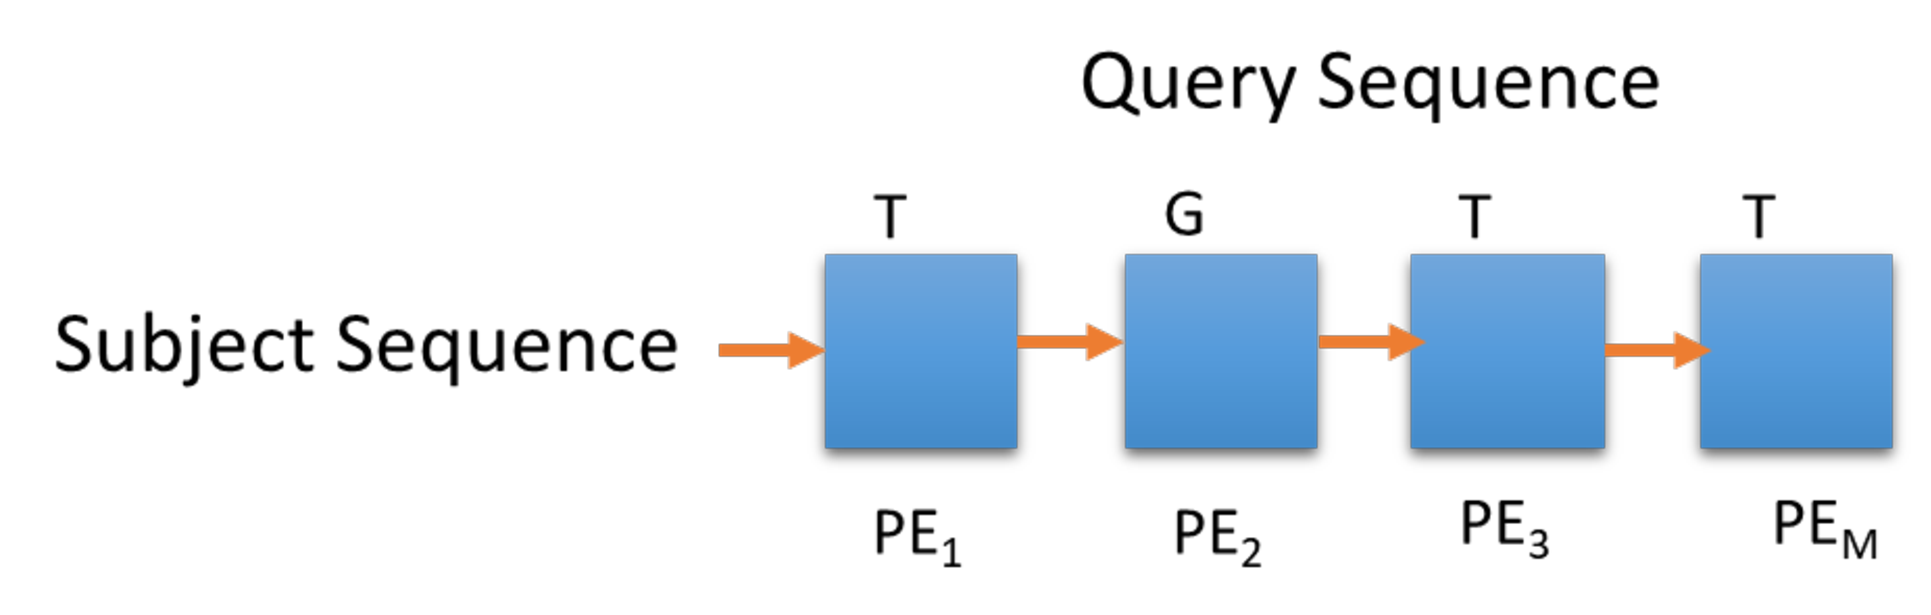
\includegraphics[width=0.7\textwidth]{fig/systollic}
    \caption{Systolic comparator on a linear processor array (based on\cite[Figure 2]{oliver_hyper_2005})}
    \label{fig:systollicarray}
\end{figure}

The design presented by \textcite{oliver_hyper_2005} also utilize the reconfigurable nature of the FPGA by providing capabilities to modify the 
individual PEs to different gap penalty functions, variation of the data width (dw), substitution width (sw) and lookup address width (lw). 

\subsubsection{Operation of the cells}

Assuming a sequence query A of length M $ A = a_1a_2 .. a_M $ and B database sequence of length K $B = b_1b_2 .. b_K $ is to be mapped on a linear array of
M PEs with affine gap penalties, then during initialization $ PE i $ would be initialized with character $ a_i $ along with corresponding
gap penalties. After this the sequence B can pass through the array in $M+K-1$ steps. In each iteration k, the values H, E and F is calculated by
each PE parallelly in single clock cycle. 

The above operation assumes that query string size and the number of PEs are equal (M) which is not often the case. The string size will vary and 
can be greater than PE array size. In this case the computation is partitioned. Considering a query string of size M and PEs having N elements,
the query string is partitioned into $ M/N $ sequences. Initially the PEs are assigned with $ i^{th} $ partition along with gap penalties and
then the processor array goes over the database sequence iteratively. After completion of iteration the PEs are updated to next partition values.
As it is apparent, loading of the new values can be time consuming and to solve this problem the PEs are extended to store k columns of the strings along
with gap penalties to avoid memory operation. The complete system design is shown in \cref{fig:systemdesign} 

\begin{figure}[h]%
    \centering
    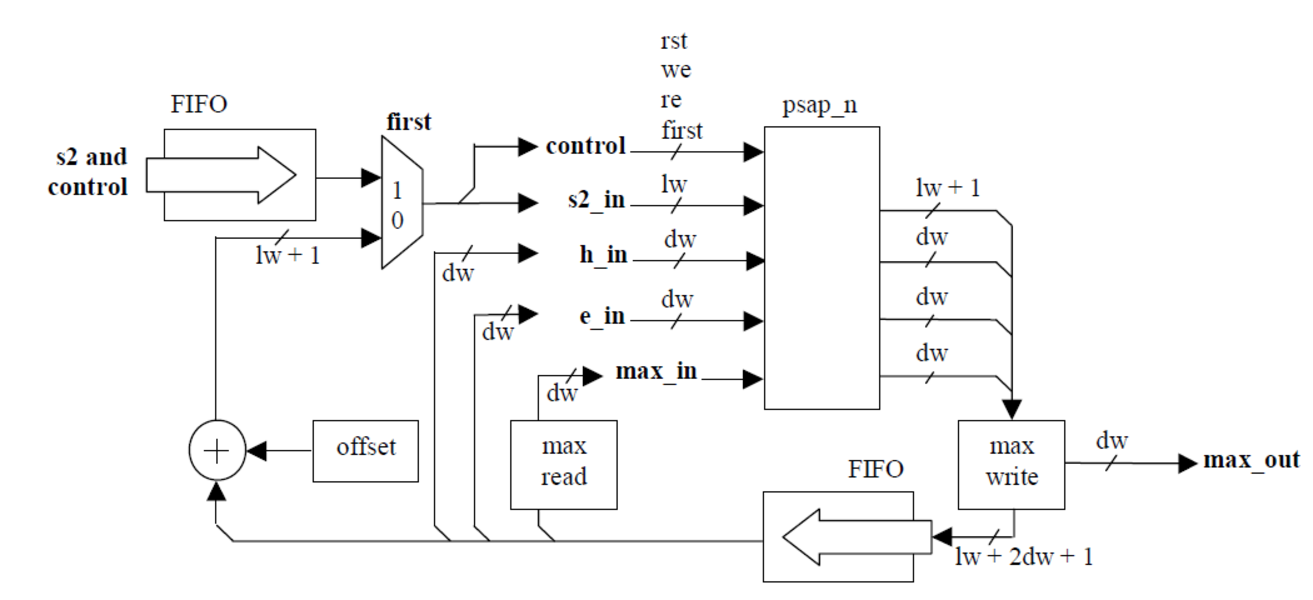
\includegraphics[width=0.8\textwidth]{fig/systemdesign}
    \caption{System design of the accelerator \cite[Figure 4]{oliver_hyper_2005}}
    \label{fig:systemdesign}
\end{figure}

\subsection{Heterogenous system design}
\label{sec:hetero}

Using the FPGA accelerator described in the \cref{subsec:fpgaaccelerator}, \textcite{meng_high-performance_2010} implemented a heterogenous system
along with other accelerators for the Smith-Waterman algorithm which can perform very fast database searches for sequence analyse.
In this section, the system would be described briefly to understand the capabilities and advantages of using a FPGA based system in a 
High performance cluster.

The system implemented by \textcite{meng_high-performance_2010} targets high-speed biological sequence analysis by utilizing different accelerators
in a distributed High performance cluster environment. The target system architecture of the system is shown in \cref{fig:hetero}. The system can
to achieve huge speed ups which will be presented in \cref{sec:eval}. The main components of the system include SIMD calculation capable
SSE2 vector computing units, FPGA coprocessor for fast processing and legacy computer system for backward compatibility.

\begin{figure}[h]%
    \centering
    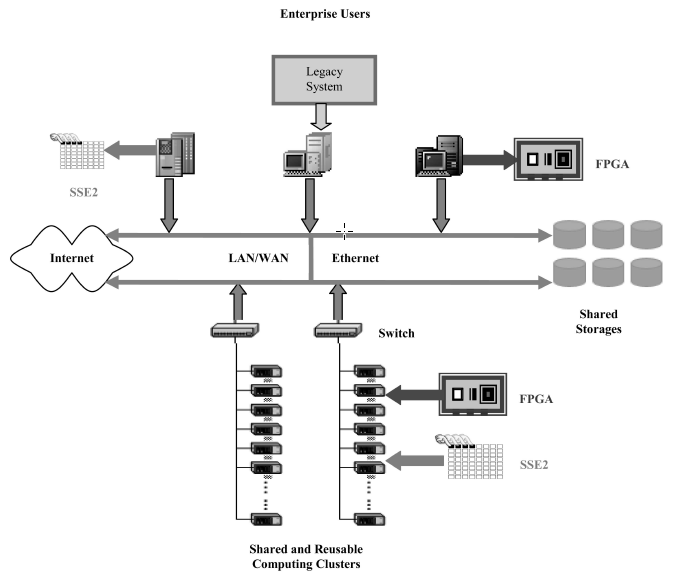
\includegraphics[width=0.6\textwidth]{fig/hetero}
    \caption{Heterogeneous computing system architecture \cite[Figure 1]{meng_high-performance_2010}}
    \label{fig:hetero}
\end{figure}

\textbf{SSE2 Vector computing} is achieved in the system by using Intel's Pentium IV and AMD Opeteron processor capable of performing SIMD calculations
on vectors using SSE2 instruction set. This allows the nodes to perform operations on 128-bit IEEE double-precision floating data types. This is used 
to perform vector calculation to compute H, E and F by transforming the calculations to utilize SIMD operations efficiently. The minor modification in
the calculation helps to bring excellent speed up to the calculation.

\textbf{FPGA coprocessor} is integrated into the host processor. The FPGA implement the systolic array design explained in \cref{fig:systollicarray}.
To control and exchange data between host and FPGA system, board specific application interface is used. As explained in \cref{subsec:fpgaaccelerator} the array calculates the 
similarity scores for the given query string and the database sequence and writes back them into the host memory. This flow can be used to
perform fine grained calculation on the FPGA and then using the scores to accumulate over the entire system by the host system. The mapping of the 
PEs.

\textbf{Legacy system} are the nodes which do not support the SSE2 instruction sets. Such system is still capable of performing
sequential processing along with some software optimization. They join the computation as worker nodes and can be used to parallelize
the computation in order to utilize the full capability of the cluster.

To efficiently utilize the heterogenous computing resources to maximize the computation capability,
specialized scheduling and load balancing schemes were developed. The communication and control between the node are done via MPI library.
An MPI master node is used to allocate workers and distribute the workload after identification and mapping the capabilities of the node.

\section{Evaluation and comparison}
\label{sec:eval}

The evaluation of the system is essential to estimate the benefits against the cost of the system. This section will present the evaluation
strategy to estimate the performance improvement for the heterogenous system described in the \cref{sec:hetero} and highlight the major
benefits from such system.

The system was evaluated using the available genome database from NCBI and EBI. Three databases were used which are described in \cref{tab:database} \cite{meng_high-performance_2010}.
Using various sources of database guarantees
the robustness of the system over variable sequence size distribution. In this evaluation only one node was equipped with FPGA co-processor
which had 119 affine PEs.
\begin{table}
    \centering
    \begin{tabular}{ |c|c|c|c| } 
    \hline
    Database format & characters & sequences\\
    \hline
    FASTA & 2,974,038 & 6,298 \\
    \hline 
    Uniref50 & 586,687,758 & 846,716 \\ 
    \hline
    month.aa & 43,531,487 & 122,650 \\ 
    \hline
    \end{tabular}
    \caption{Databases used in analysis}
    \label{tab:database}
\end{table}

\begin{figure}[h]%
    \centering
    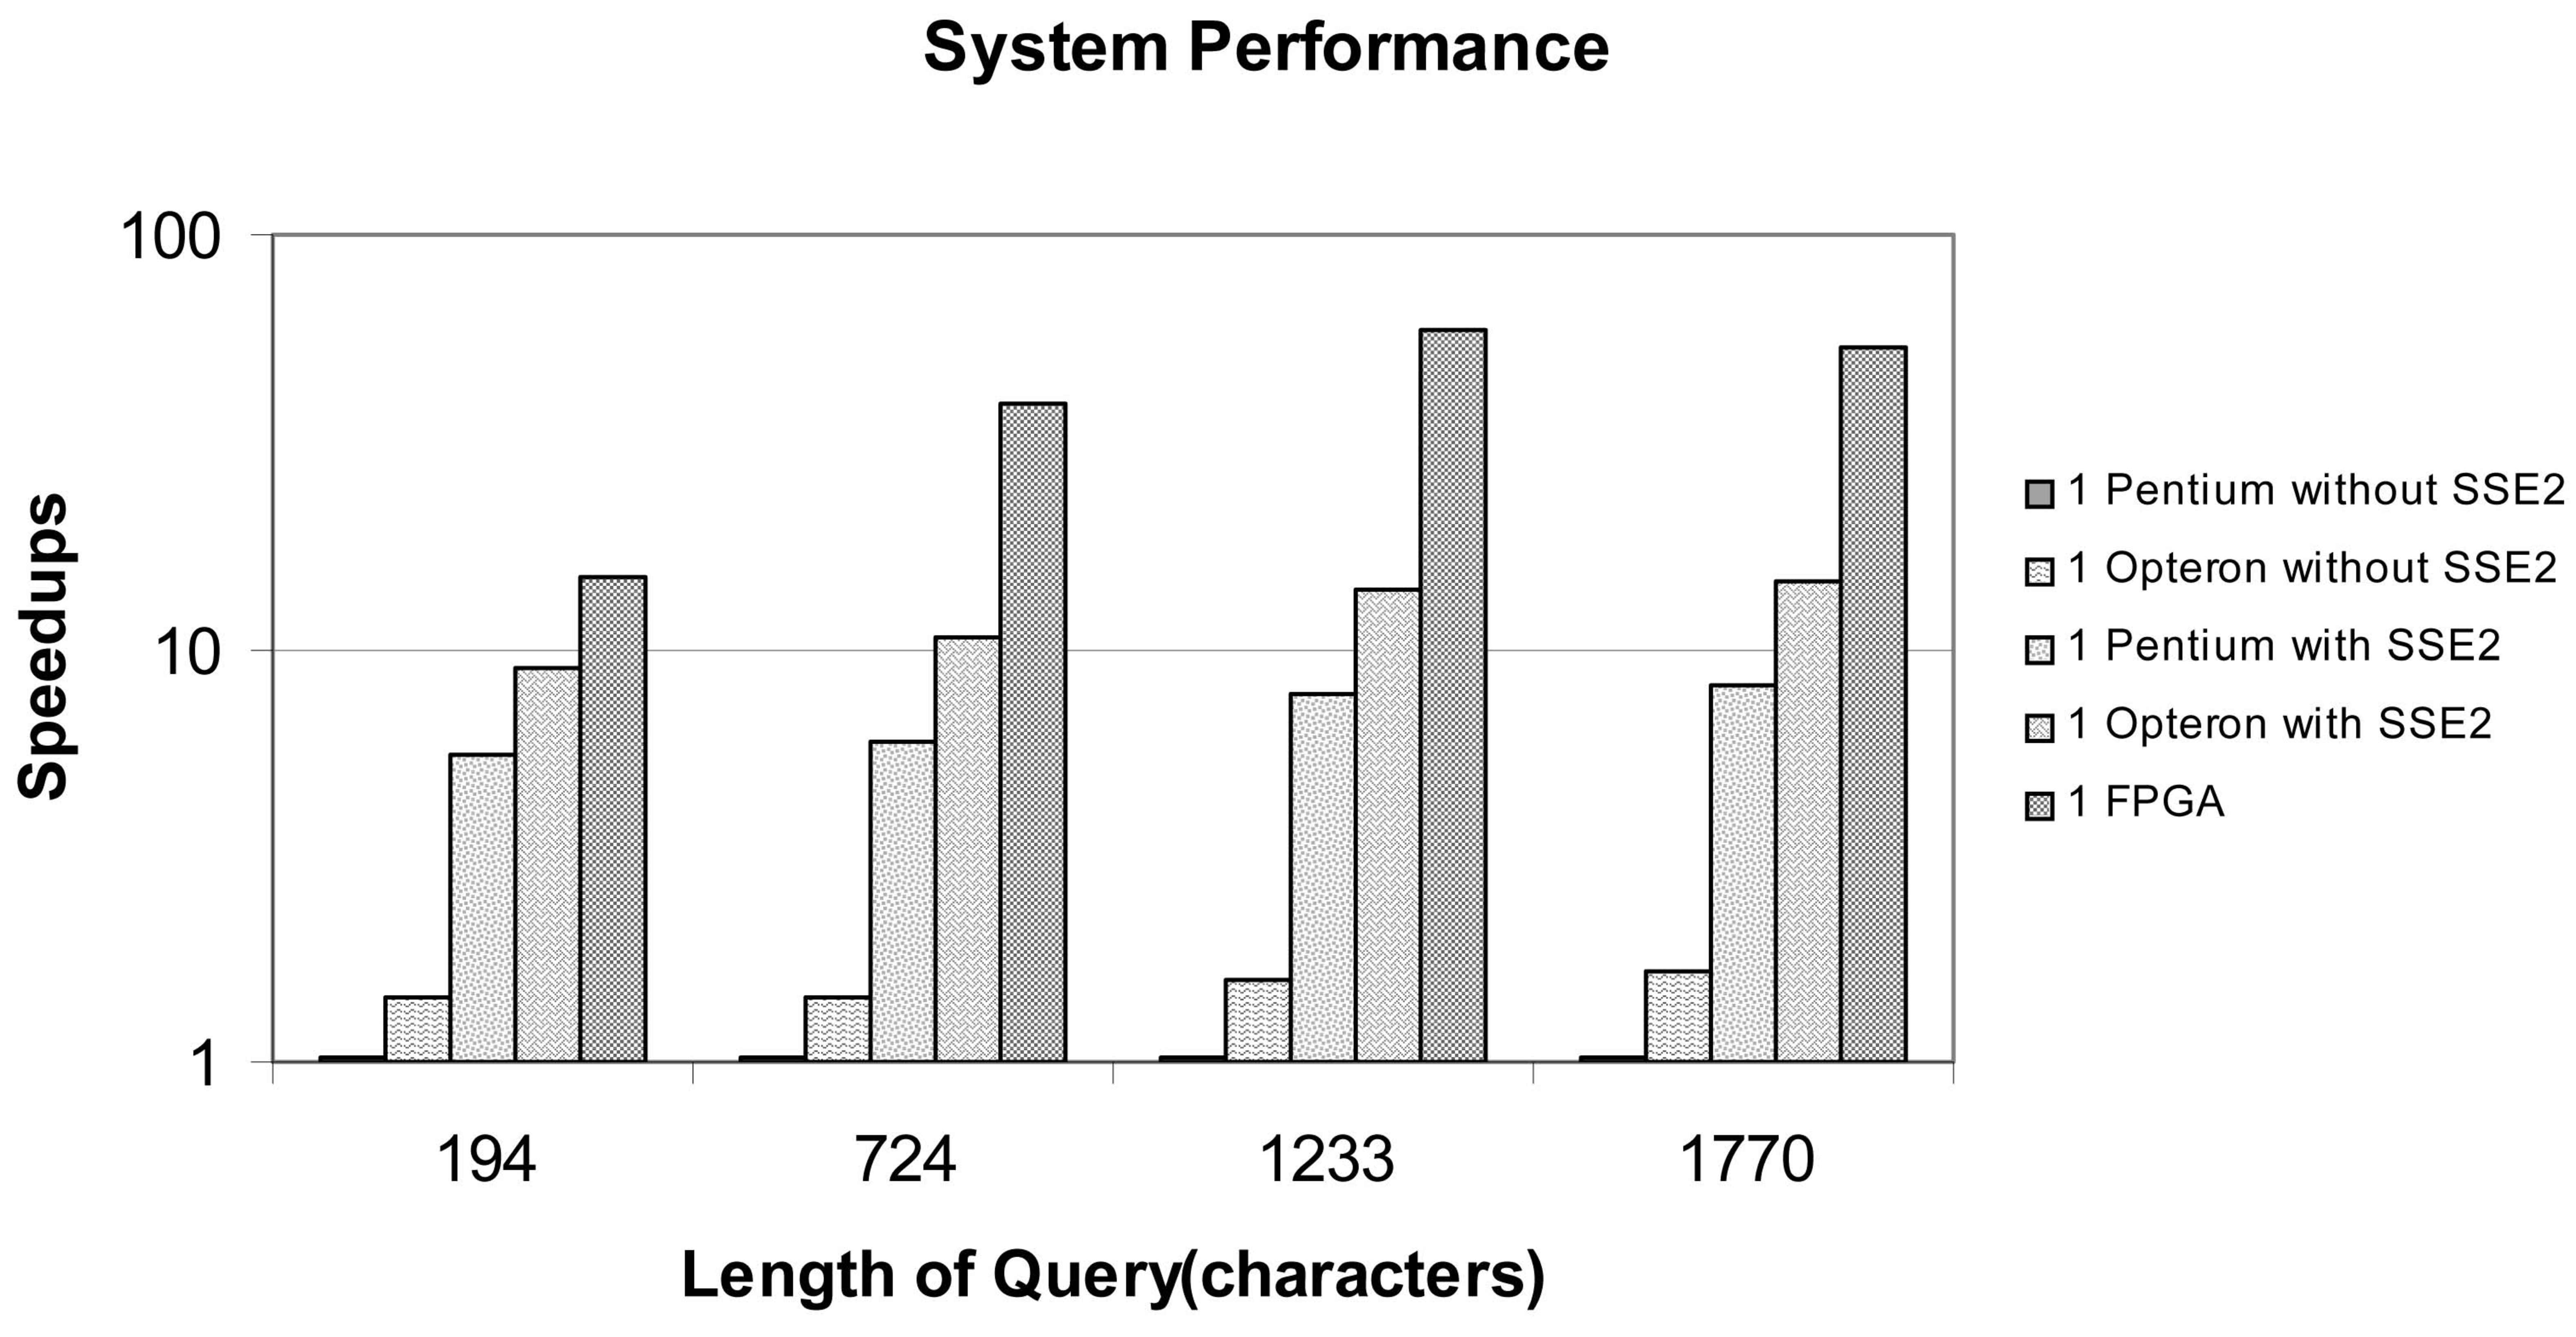
\includegraphics[width=0.8\textwidth]{fig/perform1}
    \caption{Speedup of various query lengths for various configurations \cite[Figure 10]{meng_high-performance_2010}}
    \label{fig:perform1}
\end{figure}

As shown in the \cref{fig:perform1}, a speed up of 110x is achievable with a combination of FPGA, SSE2 and MPI nodes when compared
to a serial implementation on a single Pentium IV 1.9 GHz processor. Also, tests were performed to compare the speedup achieved by the 
Heterogeneous processing element compared to uniform cluster environment with multiple similar processing nodes working using MPI.
In this case as well, for the same number of nodes a 16x speed up is observed. A comparison of the speed up for a 1233 size query on month.aa and 
uniref50 database is shown in \cref{fig:perform2} to show the speed ups for different worker nodes sizes.

\begin{figure}[h]%
    \centering
    \subfloat[month.aa]{\label{fig:perform2a}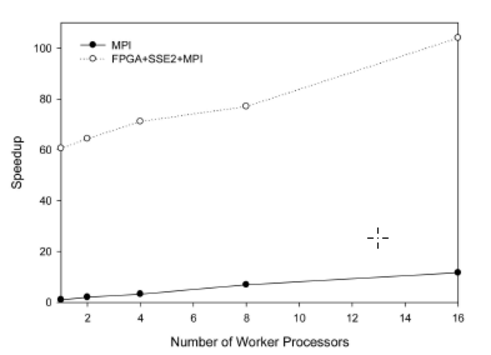
\includegraphics[width=0.5\textwidth]{fig/perform2a}}
	\subfloat[uniref50]{\label{fig:perform2b}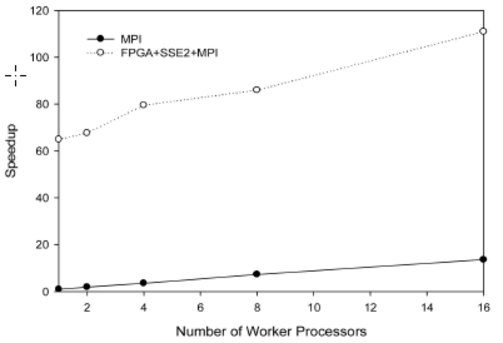
\includegraphics[width=0.5\textwidth]{fig/perform2b}}
    \caption{Performance comparison of heterogeneous \cite[Figure 12 (e,f)]{meng_high-performance_2010}}
    \label{fig:perform2}
\end{figure}

\section{Conclusion and Future work}
\label{sec:concl}

This paper introduces the various bioinformatic application and algorithm which are popular in the domain along with the optimization
which has been done using FPGA and HPC system to achieve high-speed up. As it is shown, a single FPGA coprocessor
possess very high potential for accelerating the algorithmic calculation required for the sequence analysis by a factor of 16. FPGA based 
acceleration has been a prime research area in the bioinformatic community and the capabilities demonstrated in this paper with a heterogeneous
system makes it very suitable for future. Various researches have been carried out to accelerate other algorithms such as BLAST using
specific implementations.

Currently various organizations provide products which are based on FPGA and can be integrated in the existing HPC system to provide the additional accelerations.
\emph{Timelogic}\footnote{\url{http://www.timelogic.com/}} provides DeCypher\footnote{\url{http://www.timelogic.com/catalog/755/decypher}} suite which include
hardware accelerators for Smith-Waterman (\emph{DeCypherSW\texttrademark}), BLAST (\emph{Tera-BLAST\texttrademark}) and HMM (\emph{DeCypherHMM\texttrademark})
which can be used to accelerate the genome analysis. Similarly, there are various other accelerators and projects which are aimed at integrating the FPGA coprocessor
into existing HPC systems or creating new ones to benefit from this acceleration.

\begin{figure}[h]%
    \centering
    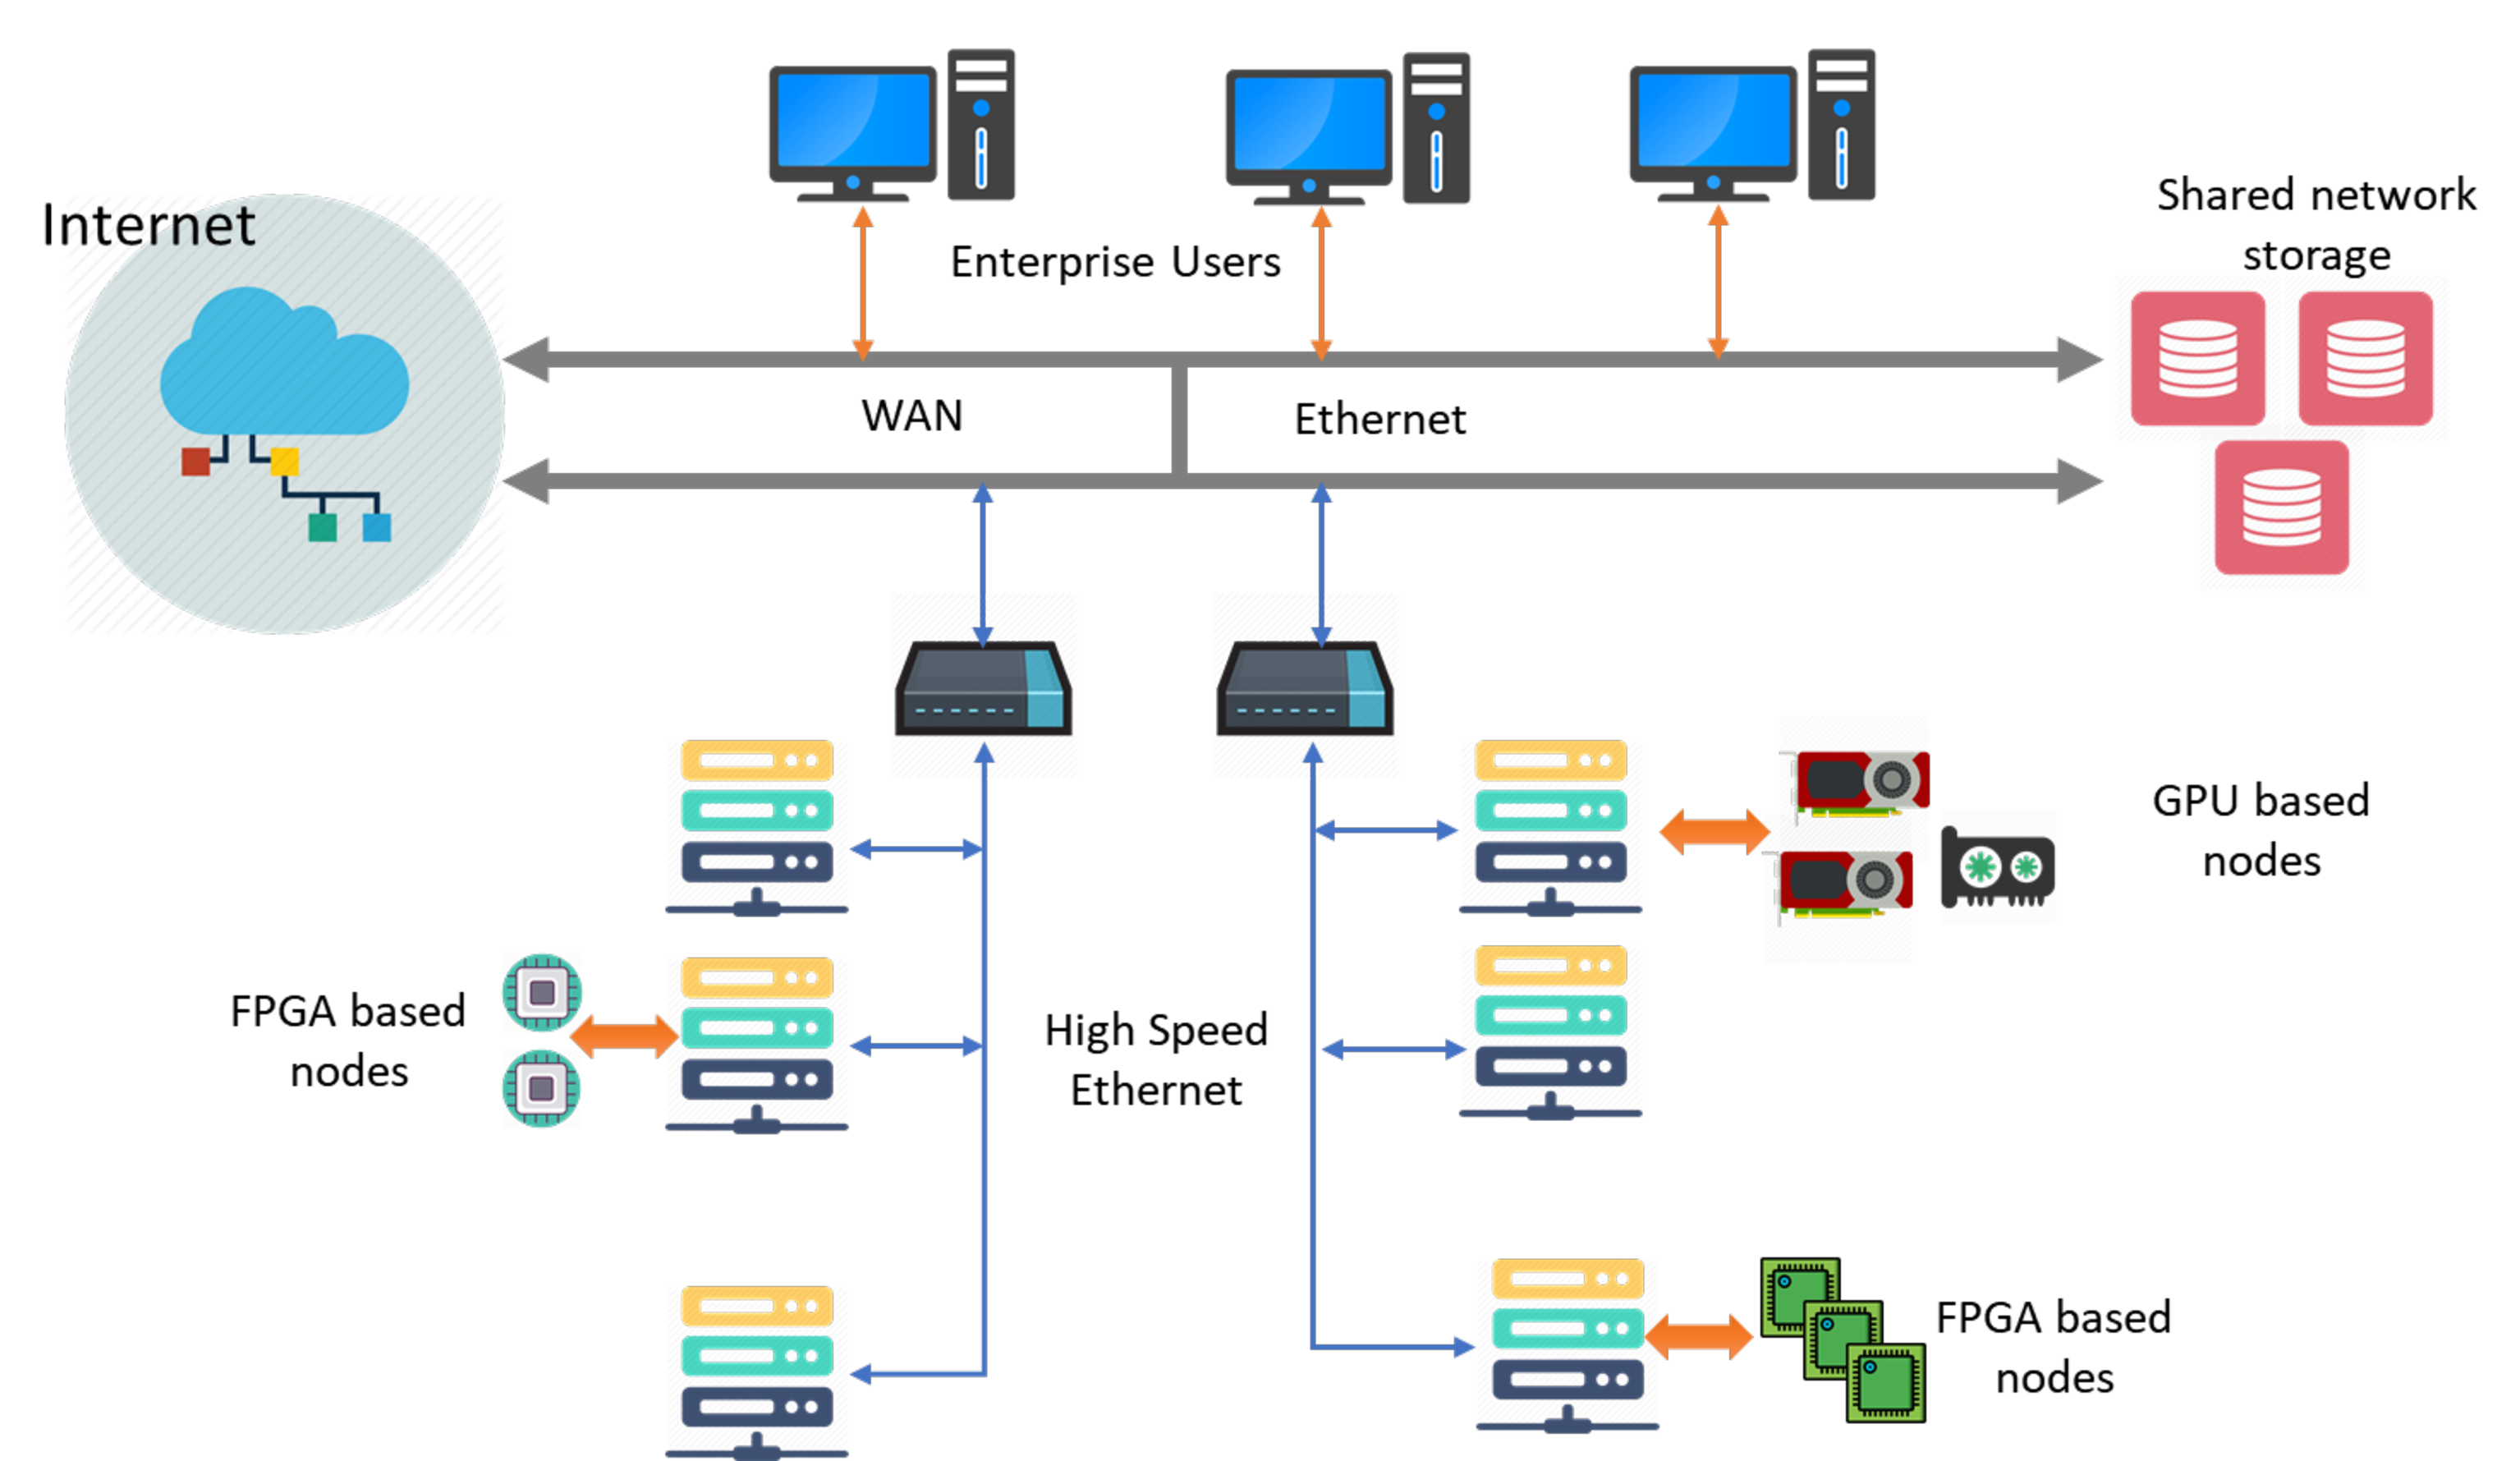
\includegraphics[width=1.0\textwidth]{fig/heterosystem}
    \caption{Futuristic Heterogeneous High performance system}
    \label{fig:futuresys}
\end{figure}

Such designs would allow in future to develop highly powerful and parallel system as shown in \cref{fig:futuresys}
which would consist different types of processing nodes and would be able to perform fast comparisons on sequences
for providing real-time results. Real-time processing would allow using the technologies to find treatments for diseases
faster, also it would be possible in near future to use the genome analysis tools for analyzing data in real-time and use it to
discover therapeutic remedies for many diseases and uncover many mysteries of the human and biological world. 

%% the following commands include the biliographic information (in BibTeX format) from the
%% file template.bib

\printbibliography

\end{document}
